\section{Preliminary Project}
This section provides an overview of the road management project for the province of Padova. It covers various aspects like including goals, system functions, databases, technological components, project guidelines, operational aspects, risk management, benefits evaluation and cost evaluation. 

\subsection{Goals}
To ensure the successful development, implementation and utilization of the system, the road registry and road signs management project for the province of Padova has defined specific goals. These objectives fall into two main categories: overarching goals and intermediate goals. They not only provide clear direction for our project team but also serve as quantifiable benchmarks to evaluate the project's overall success.

\subsubsection{Overarching Goals}
\begin{itemize}
    \item\textbf {Develop a complete road management system:}
    The primary goal of the project is to design, develop and implement a complete road management system based on the requirements of the province of Padova. The system will enable efficient management of the road network, including the documentation of road signals and safety devices, the inspection of road conditions and allowing citizen to report malformations on the road surface.
    \item\textbf {Ensure user-friendly access and compatibility:}
    The system should provide a user-friendly interface accessible through web browsers such as Chrome and Firefox. Then it should also support specific functionality through customized desktop GIS tools when necessary. Compatibility and ease of use are essential to ensure widespread adoption and efficient utilization by  internal office technicians and citizens.
    \item\textbf {Adhere to relevant standards and regulations:}
    The system must adhere with applicable road network management standards and regulations. It should guarantee accurate data representation and support data interchangeability using standard formats.
\end{itemize}

\subsubsection{Intermediate  Goals}
\begin{itemize}
    \item Allow efficient data management to import and export data in several formats, permitting integration with already existing datasets and the exchange with other external systems. Develop mechanism to update the network and ensure the realization of an historical archive to track the maintenance of the road network.
    \item Combine query and visualization systems to develop an optimal interrogation tool that mix together spatial and alphanumeric filters. Export query results and visualise ortophoto map as a background.
    \item Support road signs and safety devices management, implementing features to identify their conditions, including their position and attributes. Develop functionality to insert new signs or devices and remove damaged ones.
    \item Enable maintenance execution of road surfaces according to their conditions and the reports made by users. Ensure efficient maintenance to keep an accurate data collection over the years.
    \item Permit data consultation to implement features that allow to technicians to perform spatial and attribute based queries to recover information about reports made by users.
    \item Develop a reporting system for citizens to report the presence of holes on the road  with photo attachments and geographical location indications.
    
\end{itemize}

\subsection{System overview}
Here it will outlined the technologies, both hardware and software, used in desktop application and web application in the proposed system, to browse the information regarding the status of the road network for the Padova province.

\subsubsection{Database}
From the specification, it is known that the IT department uses the FOSS DBMS PostgreSQL: it is necessary to install the geography components PostGIS, in order to achieve the maintenance of the geographical information of the road status.
The goal of PostGIS will be the spatial data handling for the road registry.

\subsubsection{Desktop Application GIS System}
For the Desktop application, the system must require the compliance of the use of FOSS software as non-functional requirement, like openJUMP, based on the JAVA JTS library, along with a JDK for the JVM utilization. \\
Mininum hardware requirements for the user's terminals will be given.

\subsubsection{Web Application GIS System}
The web application is composed by the following components:
\begin{itemize}
    \item front-end application: this will be the available end-user interface to the system. The citizens will insert reports, while the technicians and the police officers will consult the status of the road status. The specialized team will insert information on the status of the road, like safety device damage or malformation of the road surface.
    Here a background map will displayed, along with the road network.
    \item back-end application: here the processing will take place: possibility of list all reports submitted, the report submission and more.
    \item database application: this part will store the information regarding the road network status.
\end{itemize}

\subsubsection{Software Requirements}
For the \textbf{openJUMP plugins} the following software technologies will be used:
\begin{itemize}
    \item \textbf{openJUMP} software with the ad-hoc developed plugins.
    \item \textbf{JAVA VIRTUAL MACHINE} used by openJUMP. 
    \item \textbf{PostgreSQL DBMS} and \textbf{DBMS connecto}r to access PostgreSQL data.
    \item \textbf{Ubuntu} as FOSS operating system in the user terminals. 
\end{itemize}

\newpage

The \textbf{Desktop Application} will utilised the following software technologies:
\begin{itemize}
    \item \textbf{PostgreSQL DBMS} and \textbf{DBMS connector} to access PostgreSQL data.
    \item \textbf{PHP interpreter} to execute the PHP back-end code.
    \item the FOSS software \textbf{Apache HTTP Server} for publicing the Web Application. 
    \item \textbf{JavaScript interpreter} for the front-end processing and for showing the background and road map.
    \item \textbf{HTML} as structure of the Web Application and \textbf{CSS} for the Web Application styling. The interpreter is the user browser.
    \item the FOSS JavaScript based library \textbf{OpenLayers}, for displaying the background map, using the FOSS map service \textbf{OpenStreetMap}.
    \item \textbf{GeoServer} with Web Map Service (WMS) to handle spatial data.
    \item \textbf{TomCat} (or other related software) application is necessary to run GeoServer on Java Container.
    \item \textbf{system firewall} and \textbf{proxy firewall} to manage unauthorized access to the internal system.
    \item \textbf{Ubuntu} as FOSS operating system used to run the Servers present in System. 
\end{itemize}

\subsubsection{Hardware Requirements}
The hardware requirements for the System are:
\begin{itemize}
    \item \textbf{Hardware for Web Server} hardware and UPS for managing access to the Web Application
     \item \textbf{Hardware for Geo Server} hardware and UPS for handling GeoServer software
     \item \textbf{Hardware for Database Server} for storing, accessing and modifying the data associated to the road network.
     \item \textbf{Hardware for Internal Server}: here will be provided functionalities for the Province Office, like shared printers.
     \item \textbf{Office terminals}: a terminal with 8 GB or RAM and base line Intel Core i5 from the $13^{th}$ generation will be enough to access the Desktop Application functionalities.
     \item \textbf{no} specifics \textbf{hardware requirements are needed by the end users} for accessing the Web Application.
\end{itemize}

\subsubsection{System Schema}

     \begin{figure}[h]
        \centering
        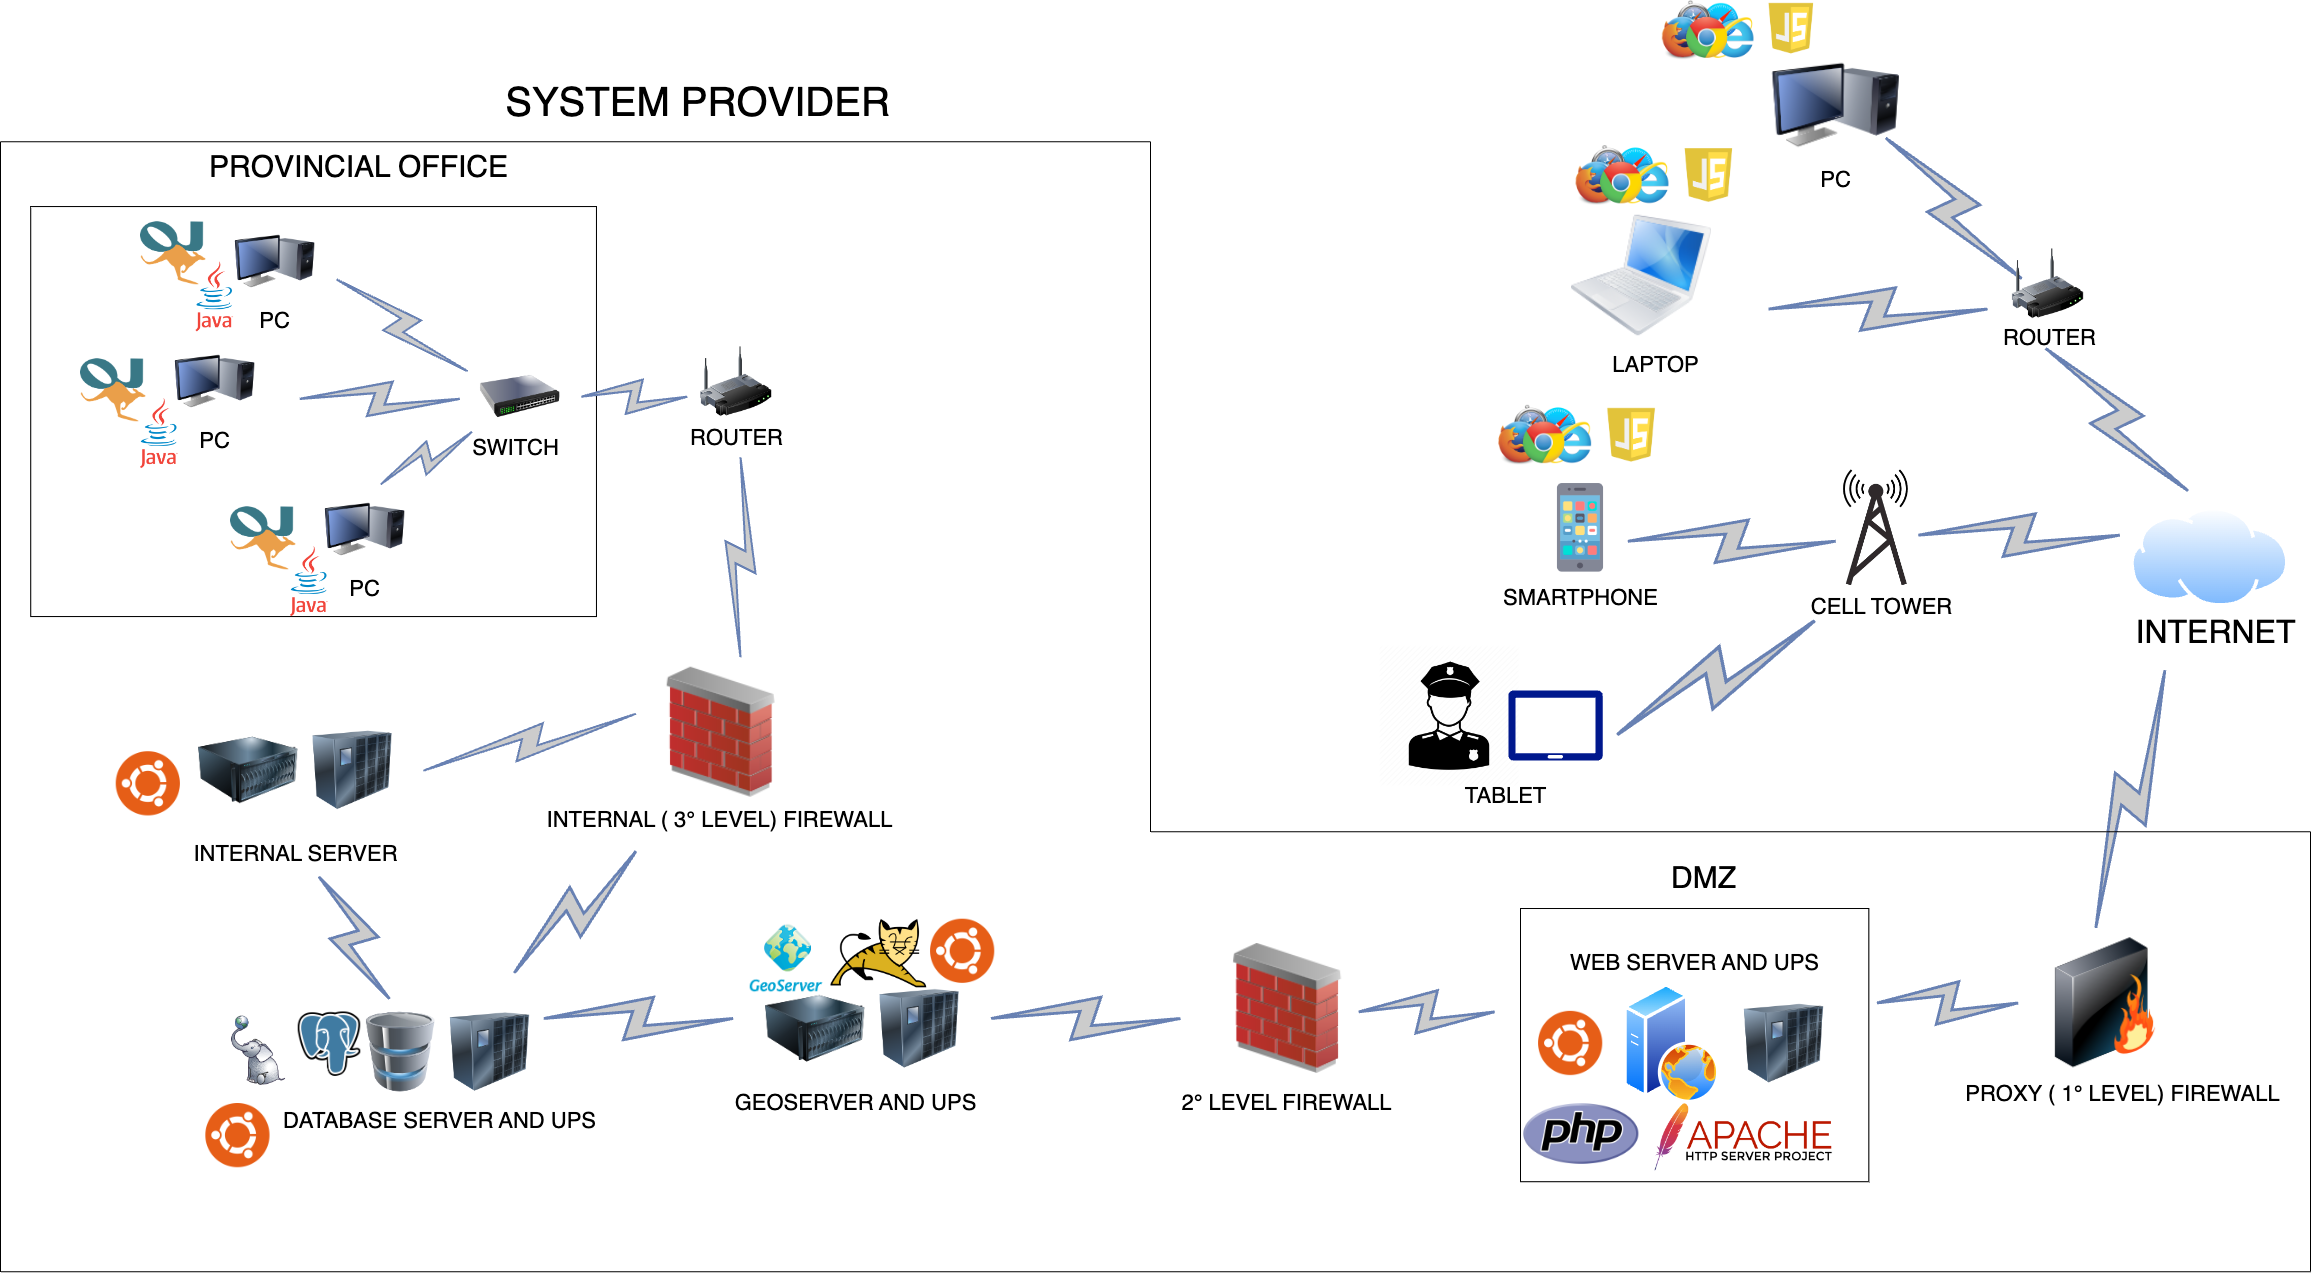
\includegraphics[width=0.7\textwidth]{images/system.png}
        \caption{System schema}
        \label{fig:yourlabel}
       \end{figure}


 Core functionalities of the System:
 \begin{itemize}
     \item \textbf{three level of firewall} for ensuring maximum security. The first level is the proxy firewall to check the incoming connection, the second one handles the access to the GeoServer and Database Server.
     The third one is used internally from the office technicians to access the servers.
     \item \textbf{DMZ} (Demilitarized Zone) is the only area accessible from the public users, hence must be protected by the proxy firewall to ensure "safe" access.
     \item \textbf{UPS} ( Uninterruptible Power Supplies) used to ensure continual power supply to the servers of the System, even when the main power supply fail.
 \end{itemize}

The Web Application is accessible through to the Web Server positioned in the DMZ zone, that is publicly available to the citizens of the Padova province. \\
On the other hand, the plugins is restricted to the employees of the provincial office in the province internal network.
 \subsection{Functionality of the System}
 In this section will be outlined the core functionalites of the Web Application and of the plugins developed for openJUMP.

 \subsubsection{Web Application}
 The Web Application developed is used by the citizens of the Padova province to signal the presence of malformations in the road network, and used by the technician of the Provincial office to visualize which reports have been submitted by the citizens. 
 \begin{itemize}
    \newpage
     \item \textbf{HOMEPAGE}
      \begin{figure}[h]
        \centering
        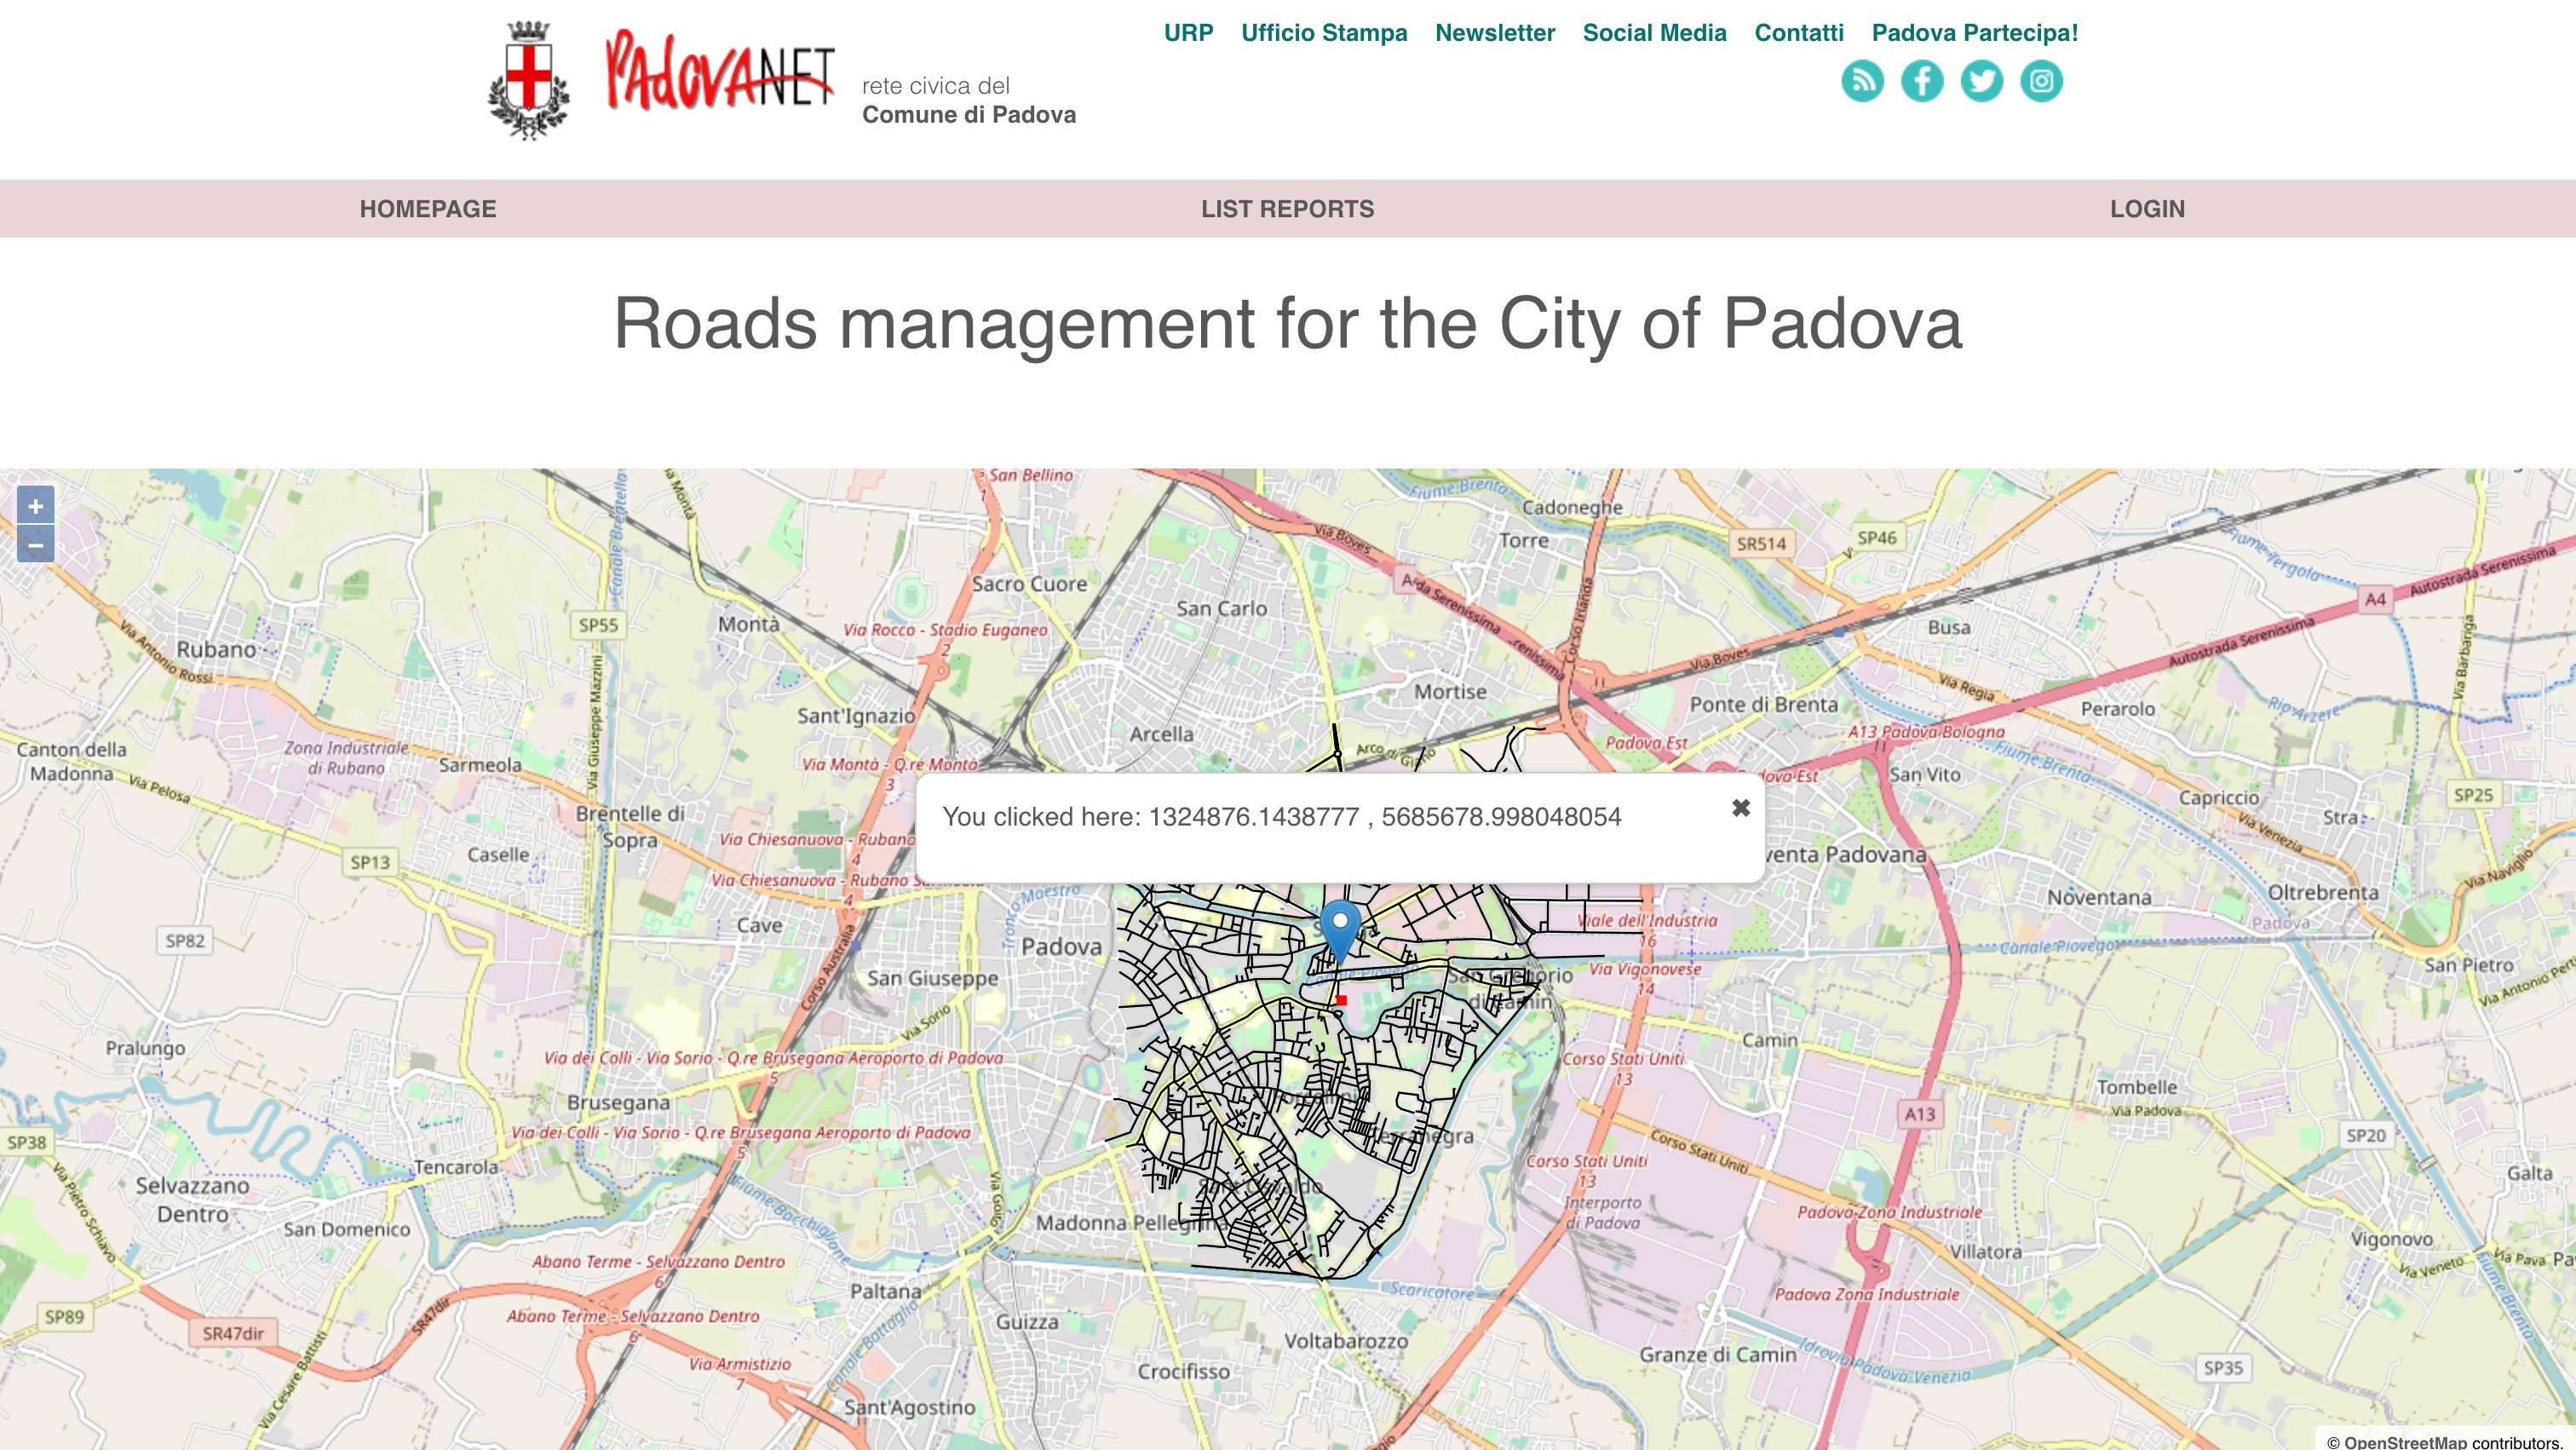
\includegraphics[width=0.7\textwidth]{images/homepage.jpeg}
        \caption{Position pin}
       \end{figure}
       \begin{figure}[h]
        \centering
        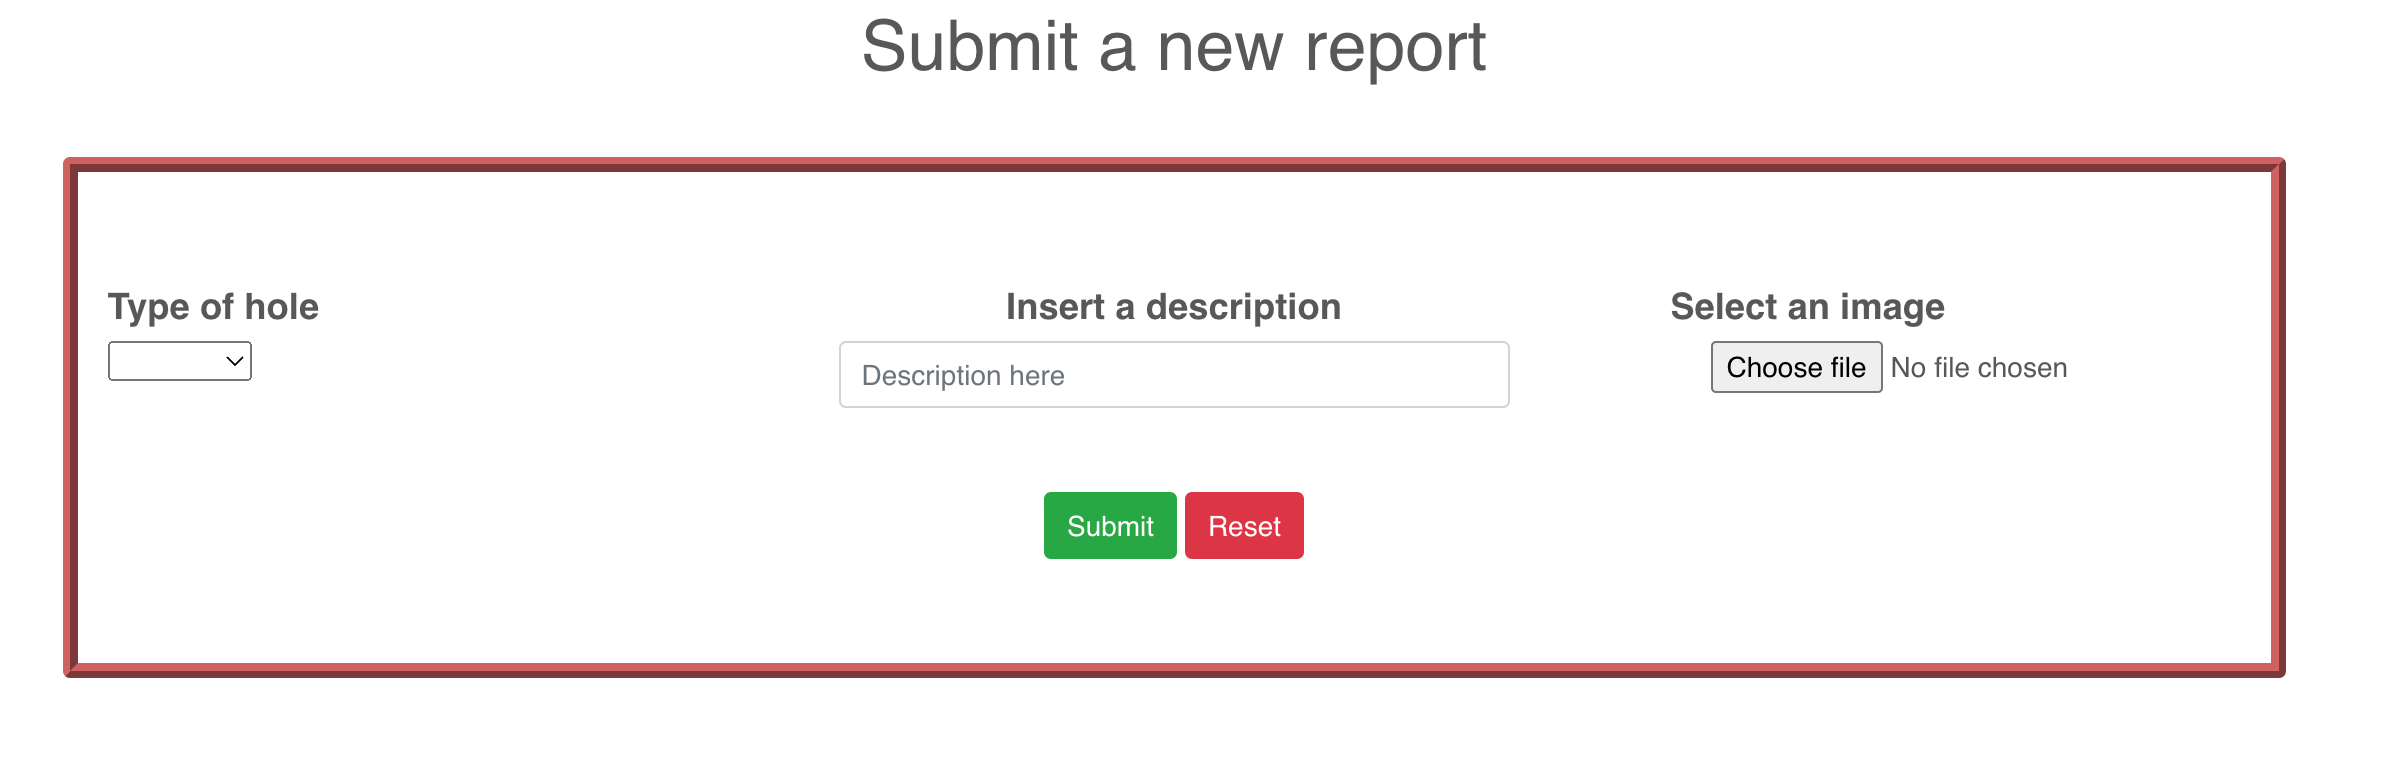
\includegraphics[width=0.7\textwidth]{images/report.png}
        \caption{Report form}
       \end{figure}

 In the homepage, it is possible to see the map displaying the road network of Padova province.
 to submit the report, the user must insert the position by clicking on the map or by using the GPS coordinate of the device.
 In the second figure is present the report form for the submission.

\newpage
    \item \textbf{LOGIN PAGE}
    
    \begin{figure}[h]
        \centering
        \centering
        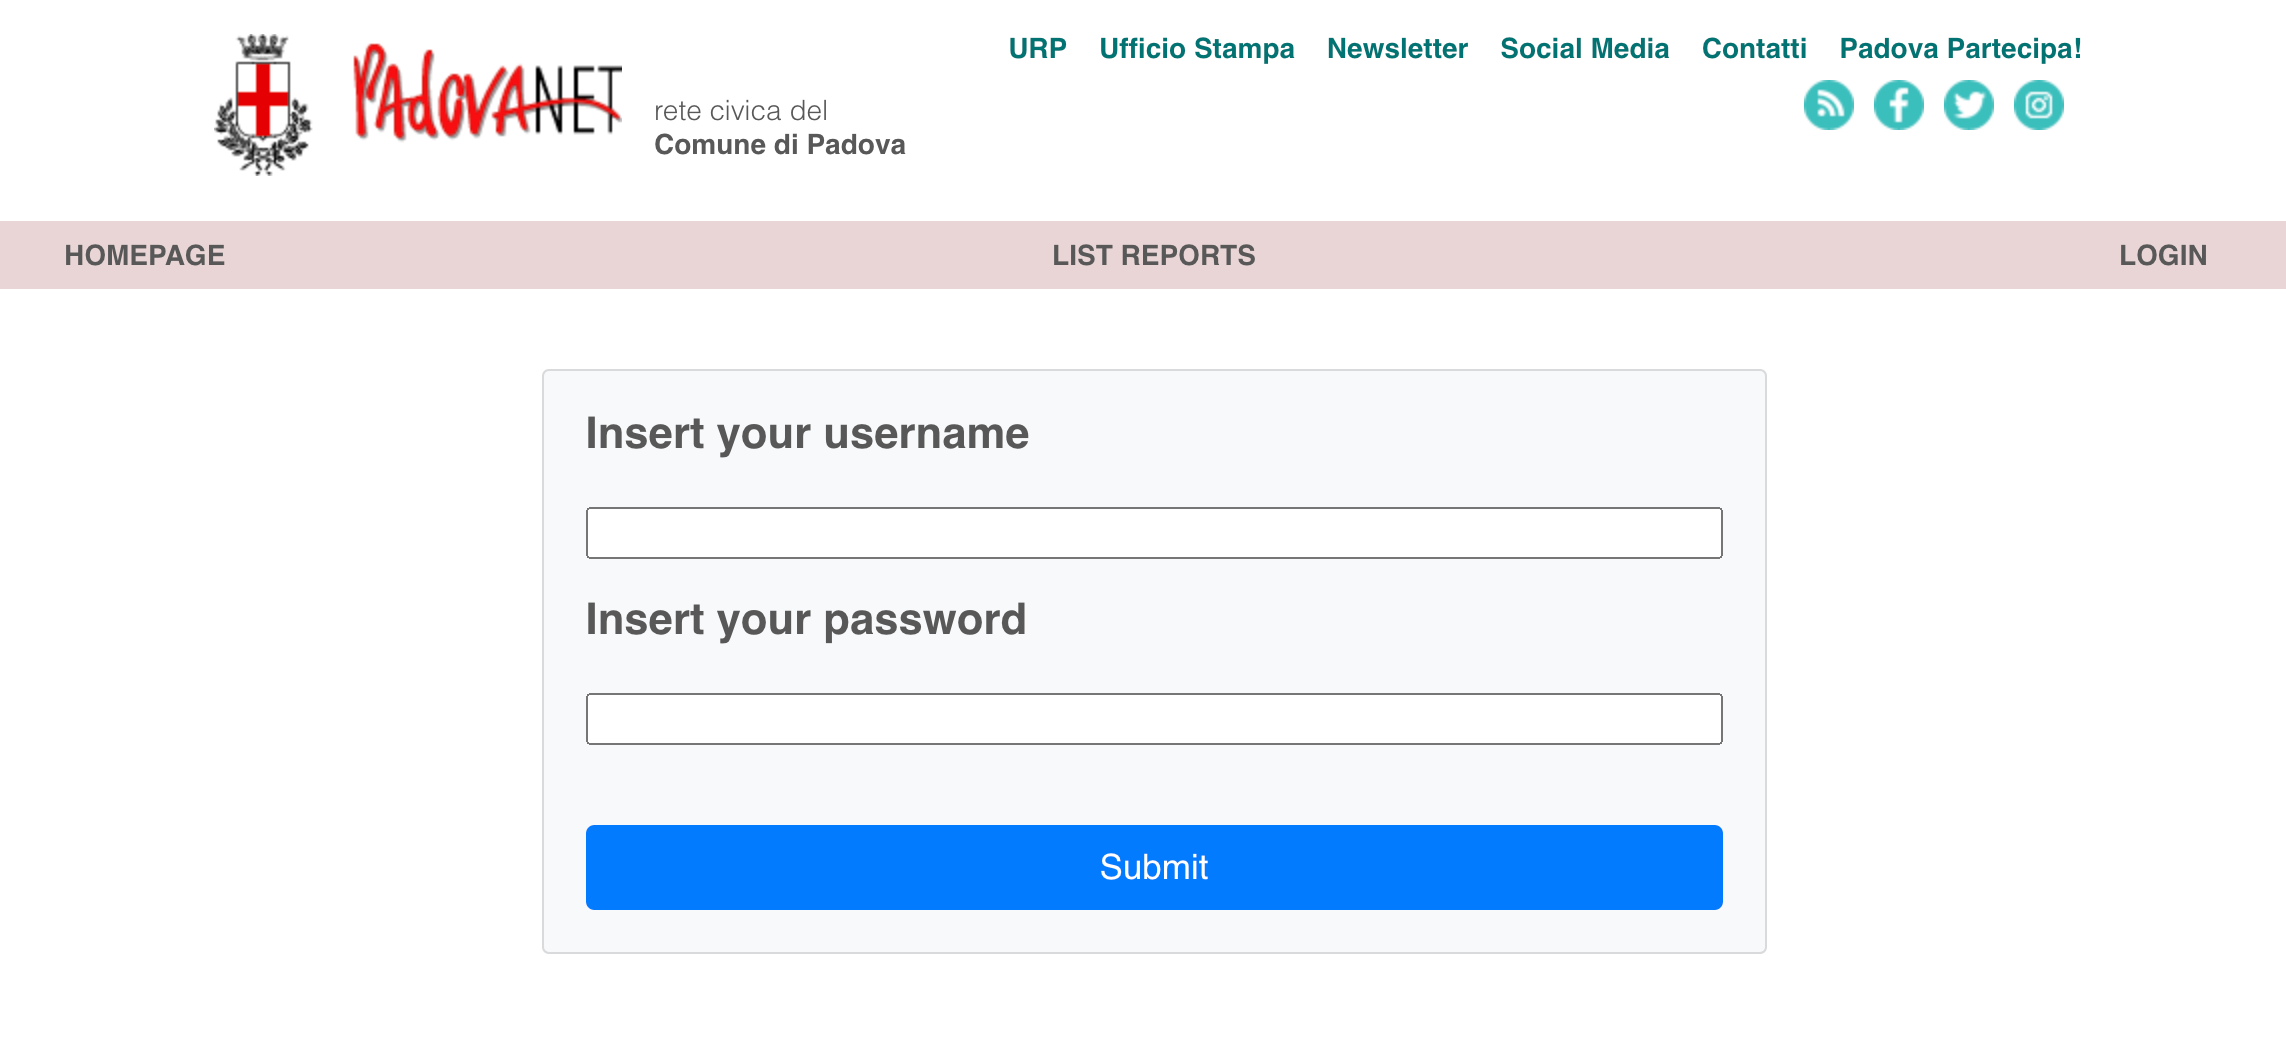
\includegraphics[width=0.7\textwidth]{images/login.png}
        \caption{Position pin}
        \label{oj_login}
    \end{figure}
    To manage unauthorized users, the system is provided of an authentication mechanism made available by the login page; only the technician of the provincial office and the police officers can access to the restricted area by performing the login operation.

    \item \textbf{LIST REPORTS}
    \begin{figure}[h]
        \centering
        \centering
        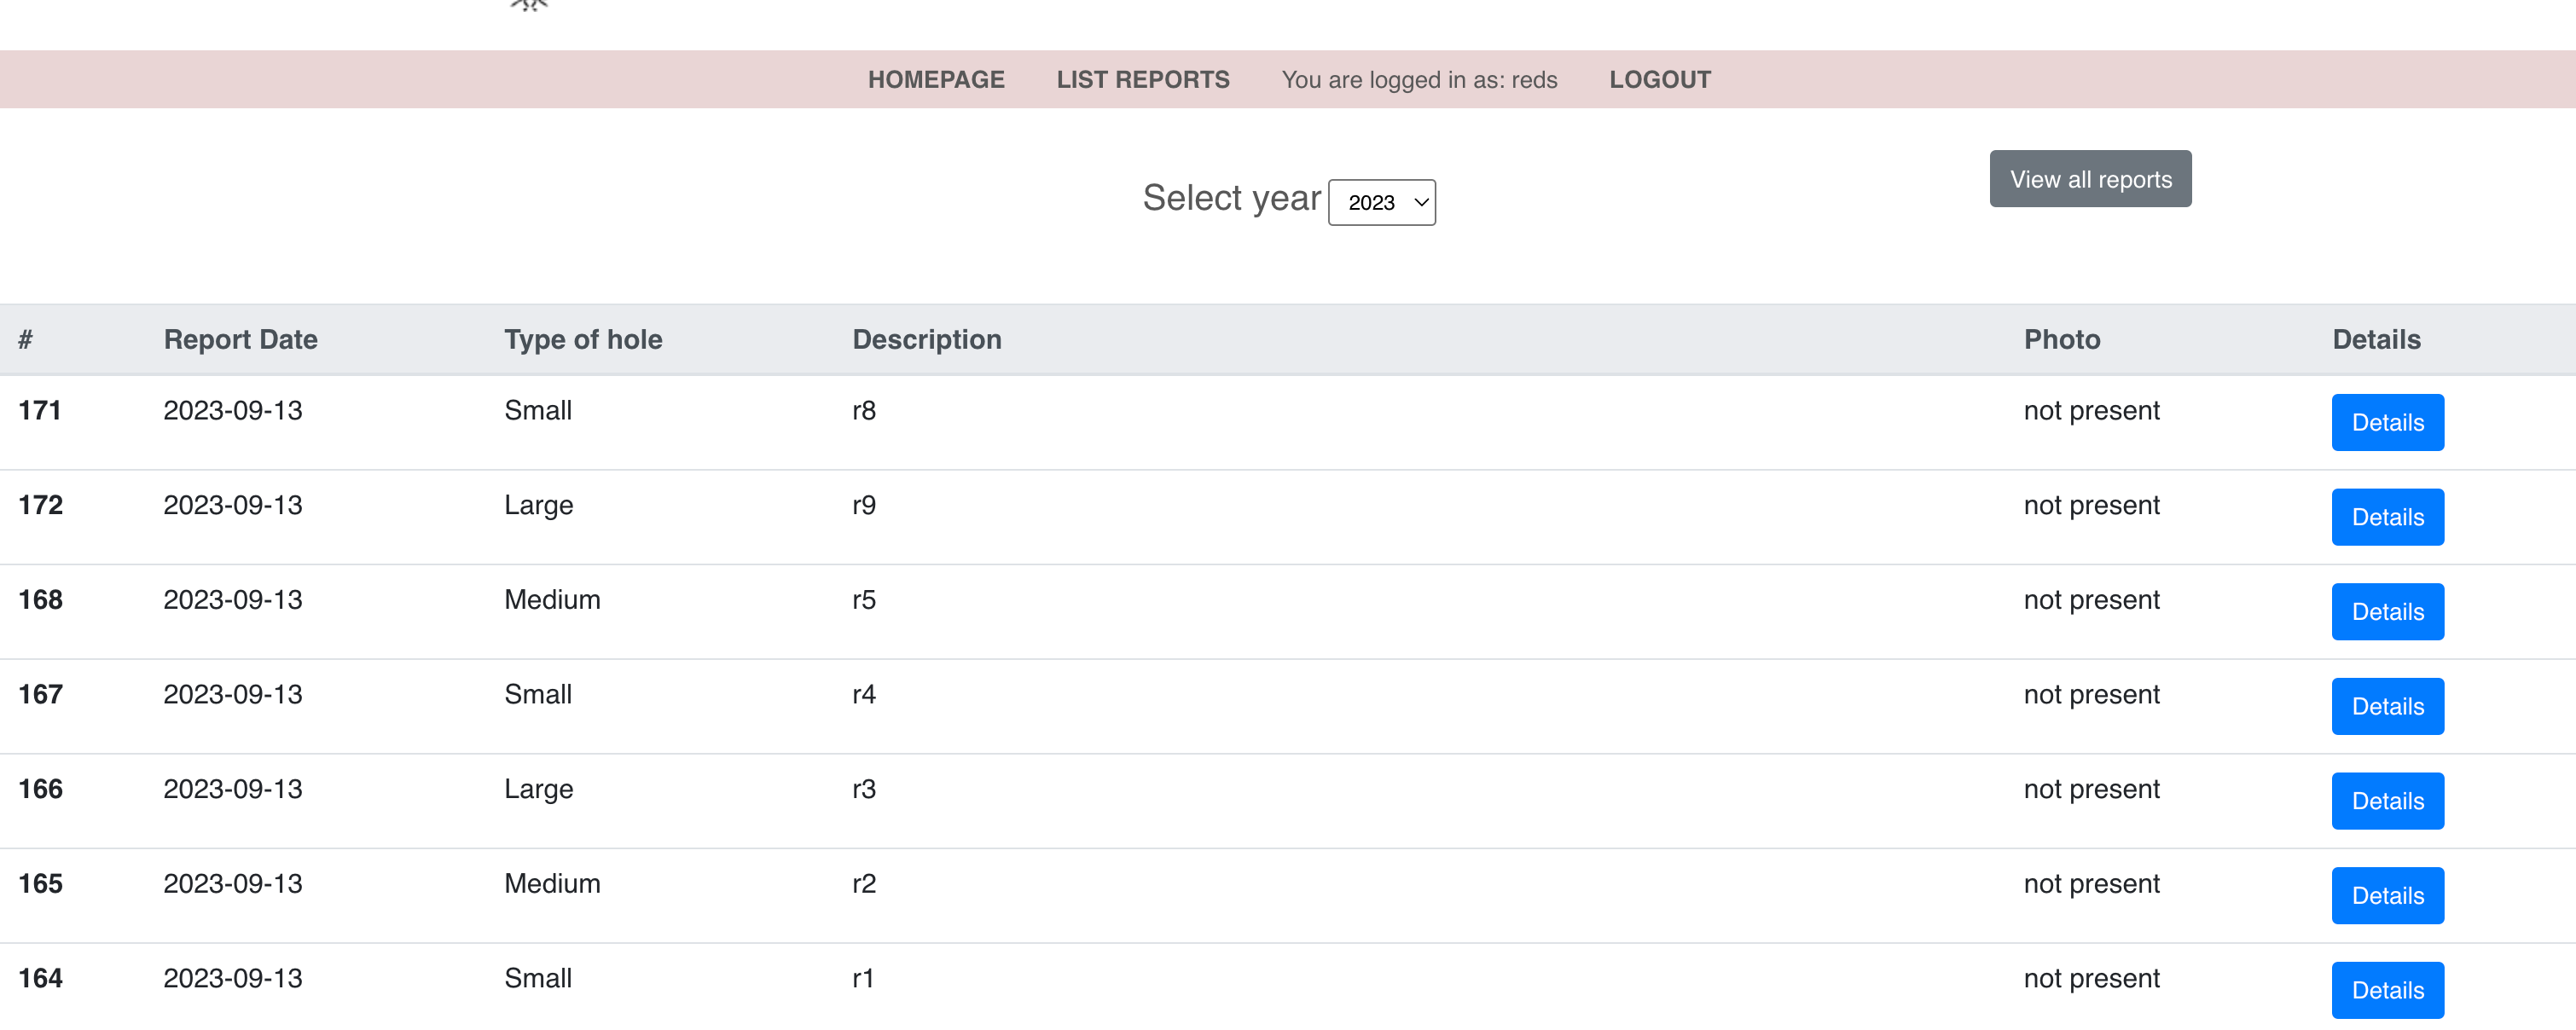
\includegraphics[width=0.7\textwidth]{images/list_reports.png}
        \caption{List reports of the selected year}
        \label{fig:yourlabel}
    \end{figure}
    In this restricted area is possible to visualize all report submitted filtered by year. From the page the operator can decide to visualize one or all reports of the selected year.

    \newpage
    \item \textbf{SHOW REPORT}
    \begin{figure}[h]
        \centering
        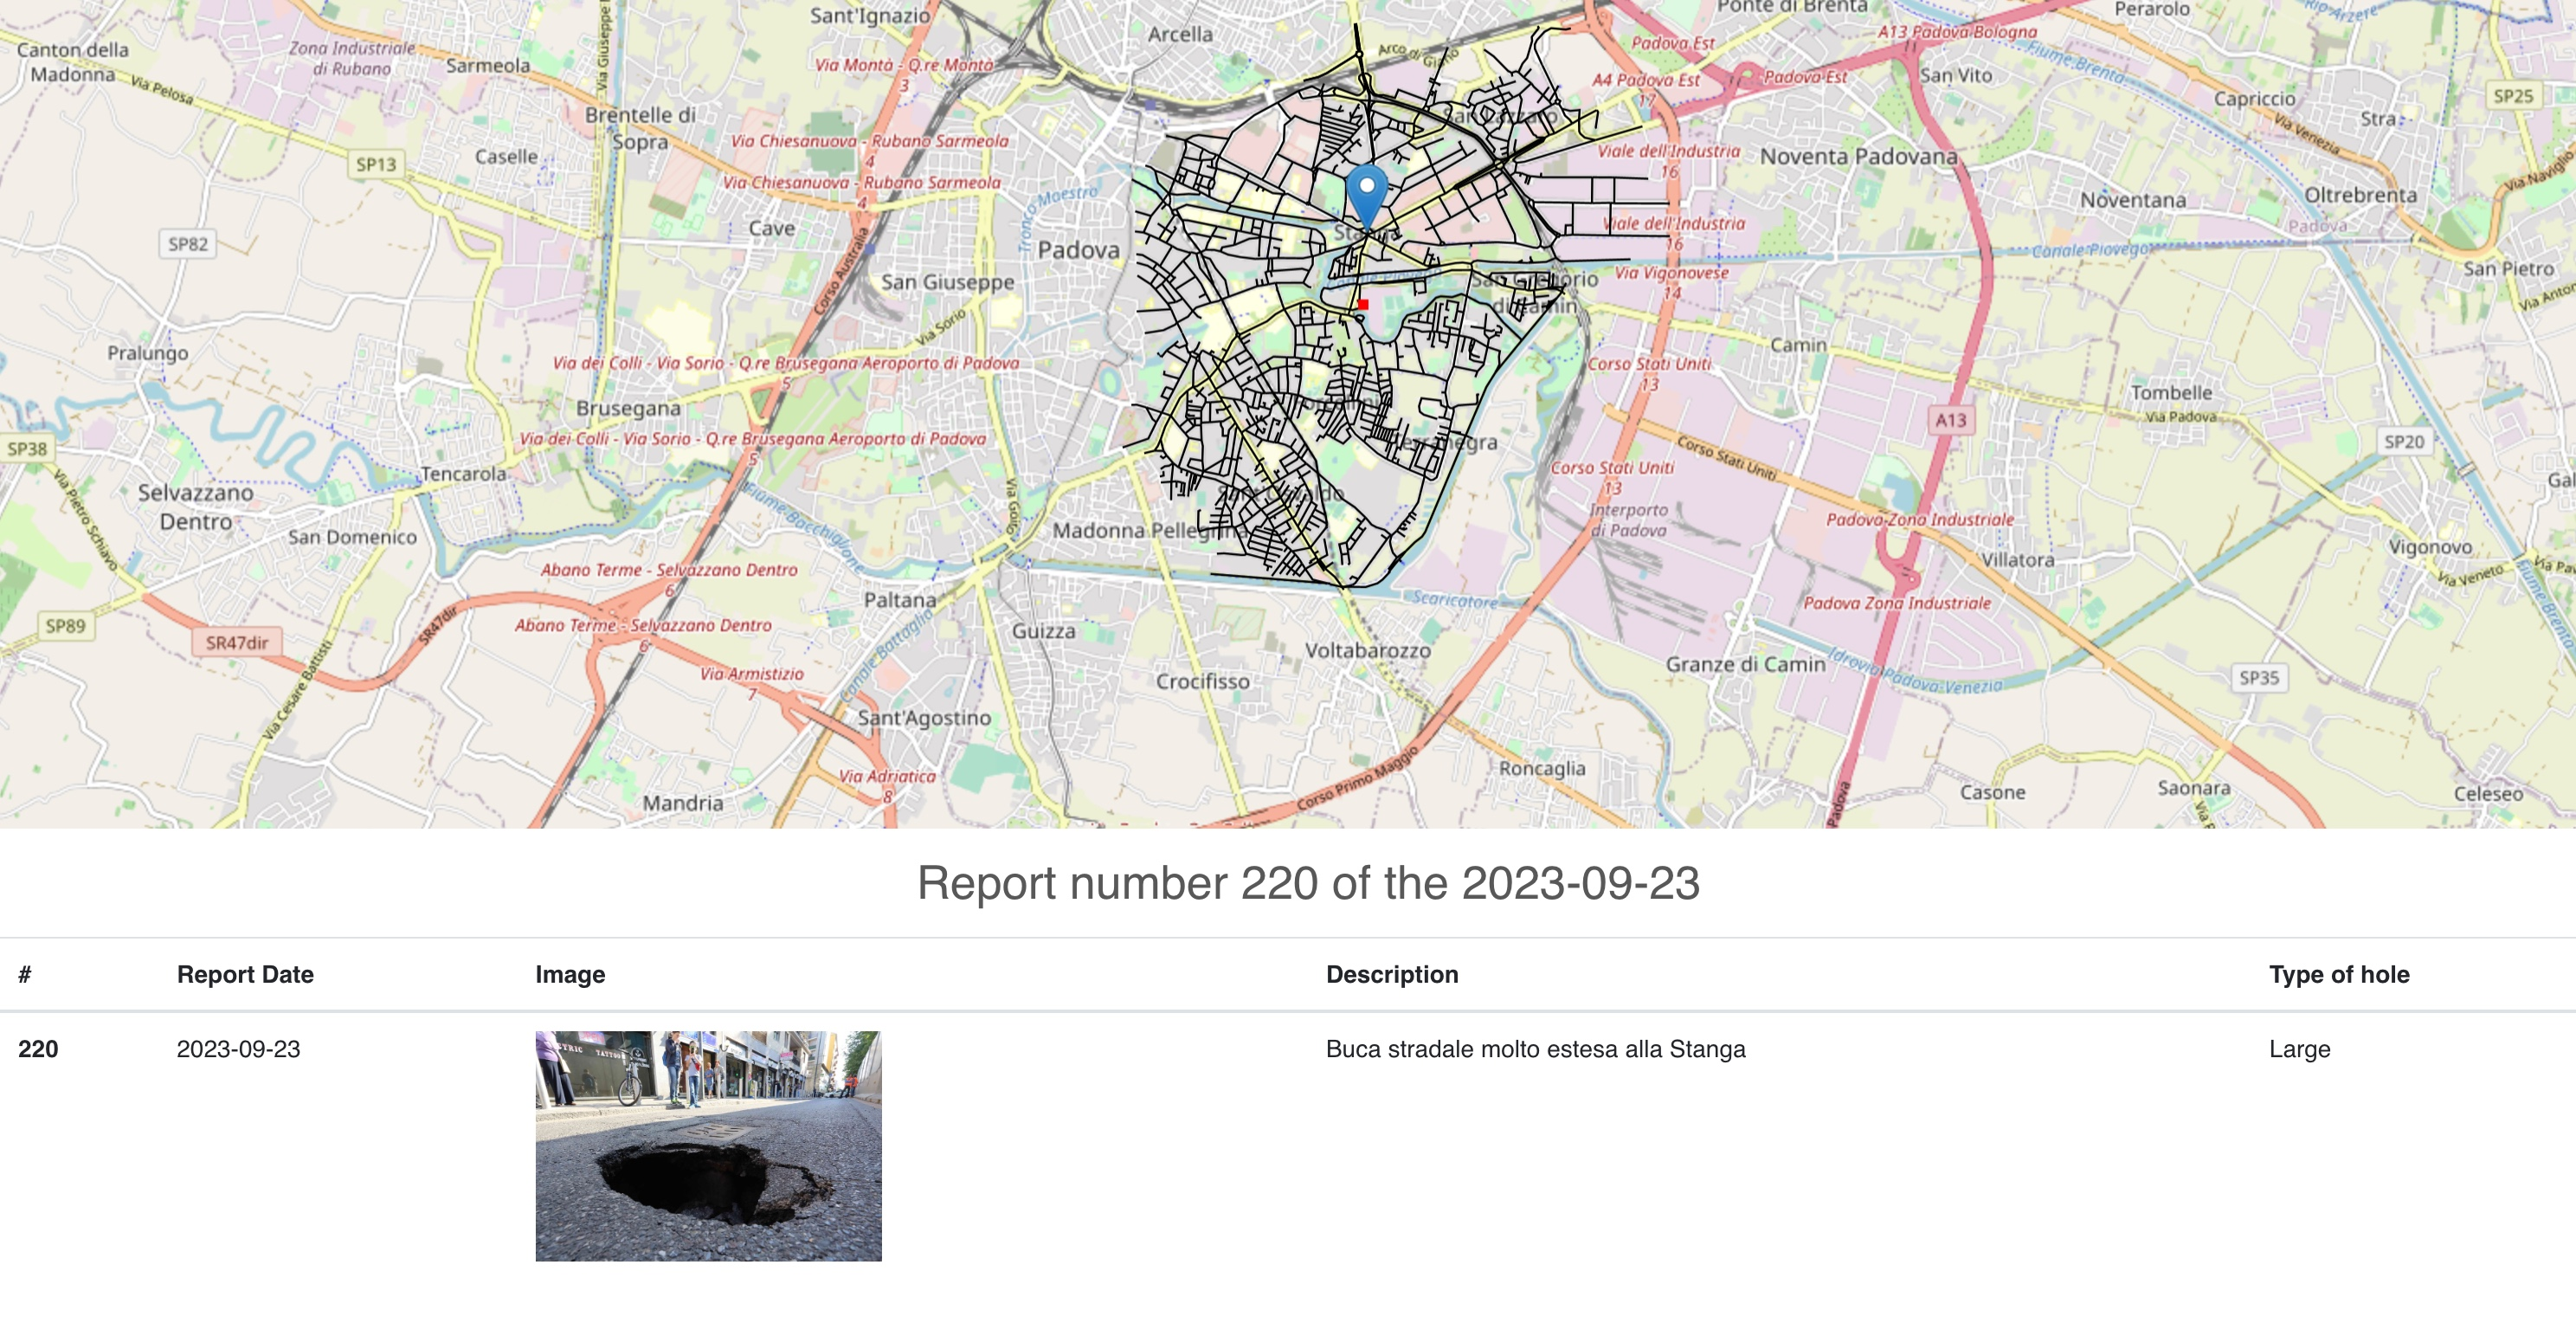
\includegraphics[width=0.7\textwidth]{images/show_report.jpeg}
        \caption{Report details}
        \label{fig:yourlabel}
    \end{figure}

    Here it is possible to visualize a specific submitted reports with its positions and all details specified by the citizens during the report submission process.
    
    \item \textbf{SHOW REPORTS}
    \begin{figure}[h]
        \centering
        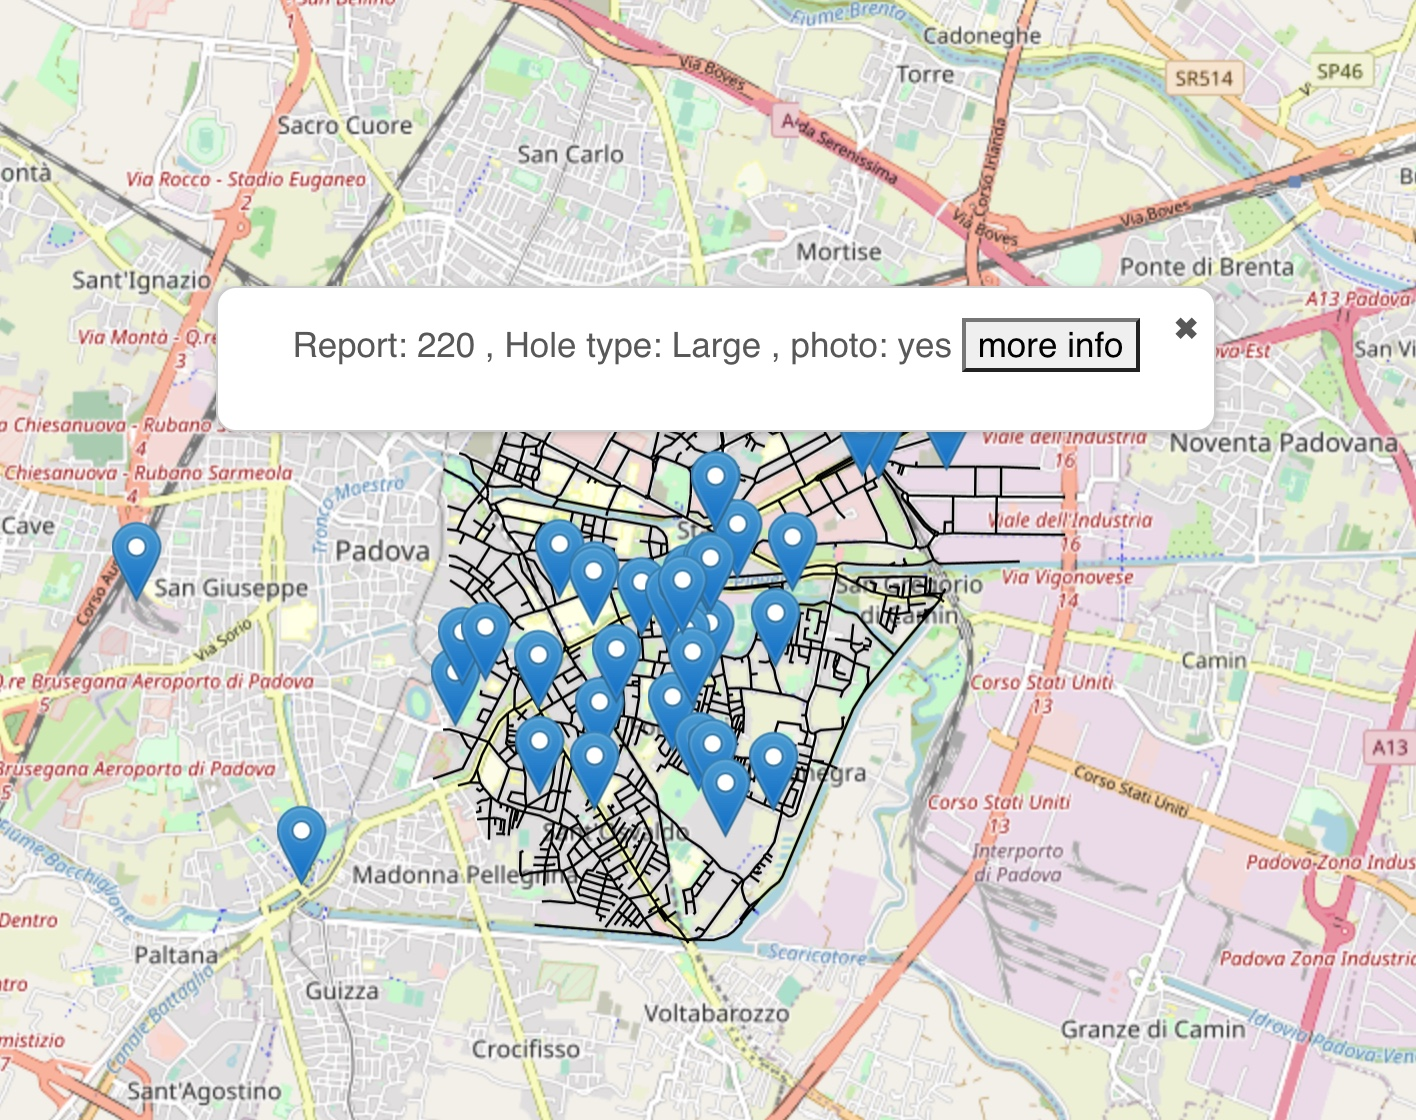
\includegraphics[width=0.7\textwidth]{images/show_reports.jpeg}
        \caption{Pins of all reports of the specified year}
        \label{fig:yourlabel}
    \end{figure}
    In the show reports page we can see all the submitted reports for the specified year, as a pin in the map. By clicking on the marker it is possible to see a short preview of the report, and by clicking the button to go to the show report page to get full informations about that report.
\end{itemize}

\newpage
 \subsubsection{openJUMP plugins}
The OpenJump plugins are used by the tehchnicians of the Provincial office to visualize where all the reports are located and then to compute a road route starting from the garage where the truck is stationed that connects the positions relative to all the reports and returns to the
starting point.
The plugin is implemented by 5 classes:
\begin{itemize}
    \item\textbf{Login.java}
    By entering username and password, it allows the user to login in the system to use the plugins. It is responsible for creating the login form. 
     \begin{figure}[h]
        \centering
        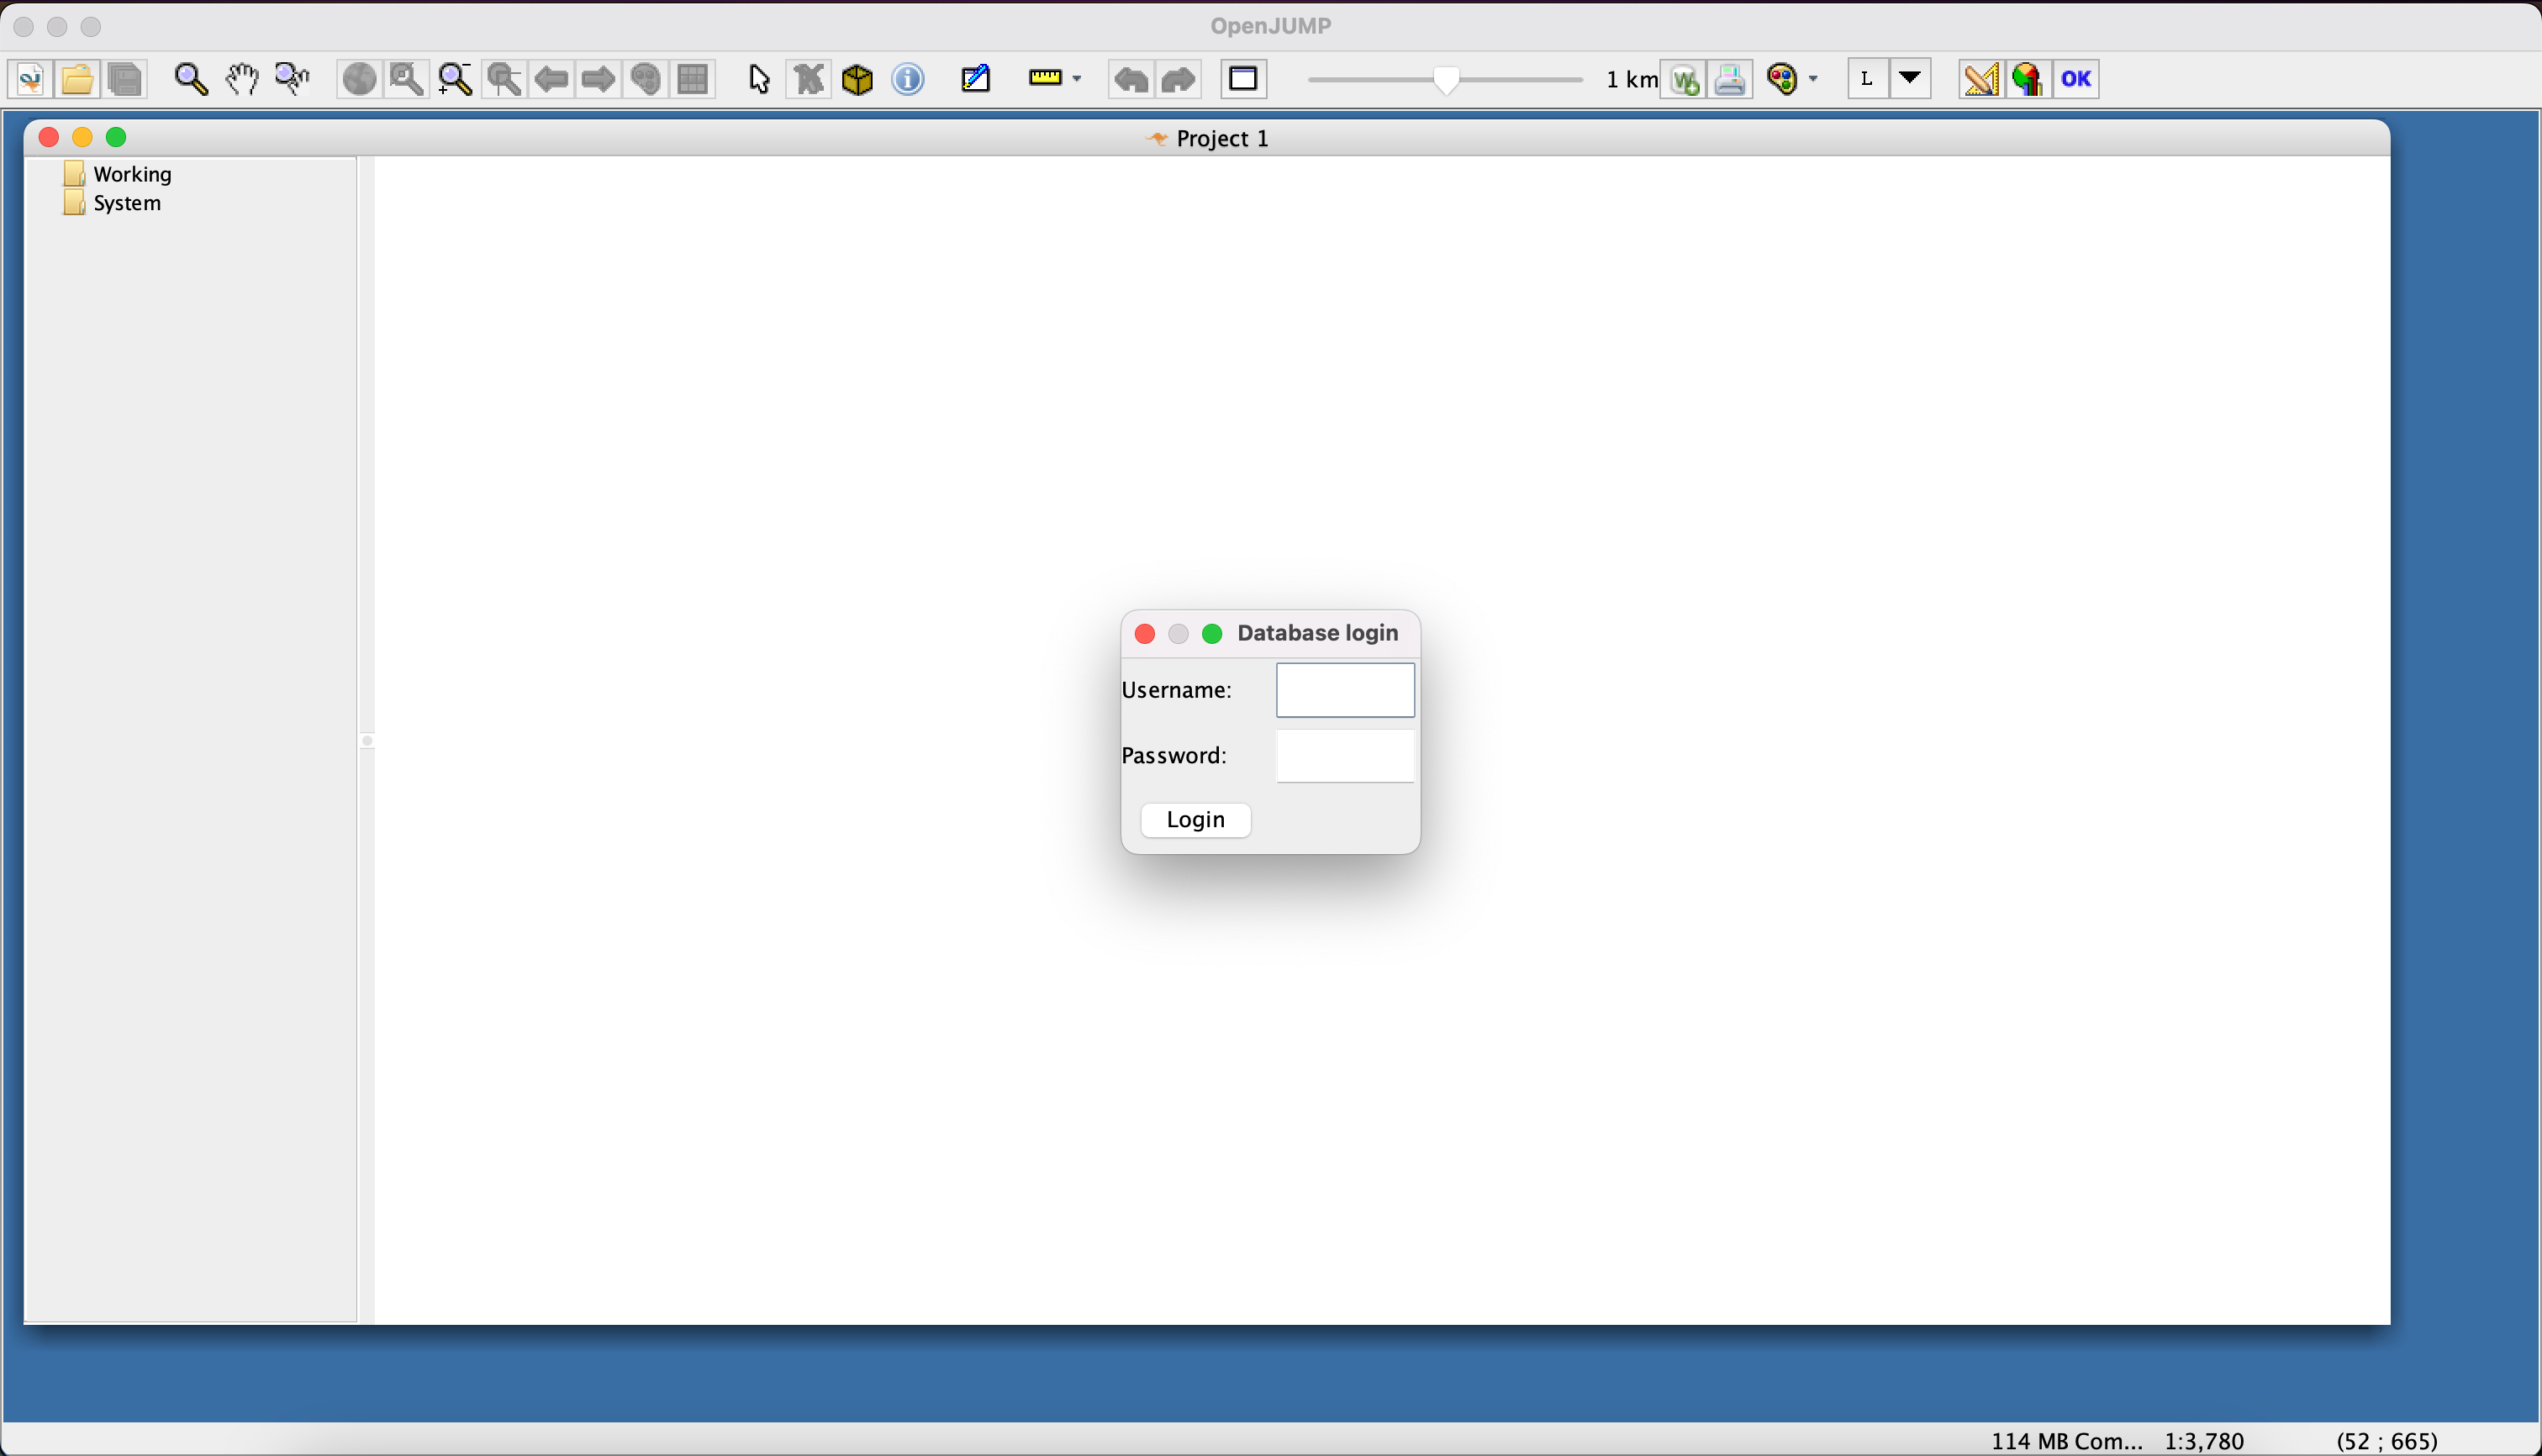
\includegraphics[width=0.8\textwidth]{images/oj_login.png}
        \caption{Login form}
        \label{ER}
 \end{figure}


    \item\textbf{Database.java}
    It connects the plugin to the database. Then it also implements two methods to extract reports information and shed position.

    \item\textbf{Plug.java}
    It loads all the reports received and shows them on the screen.
    \begin{figure}[h]
        \centering
        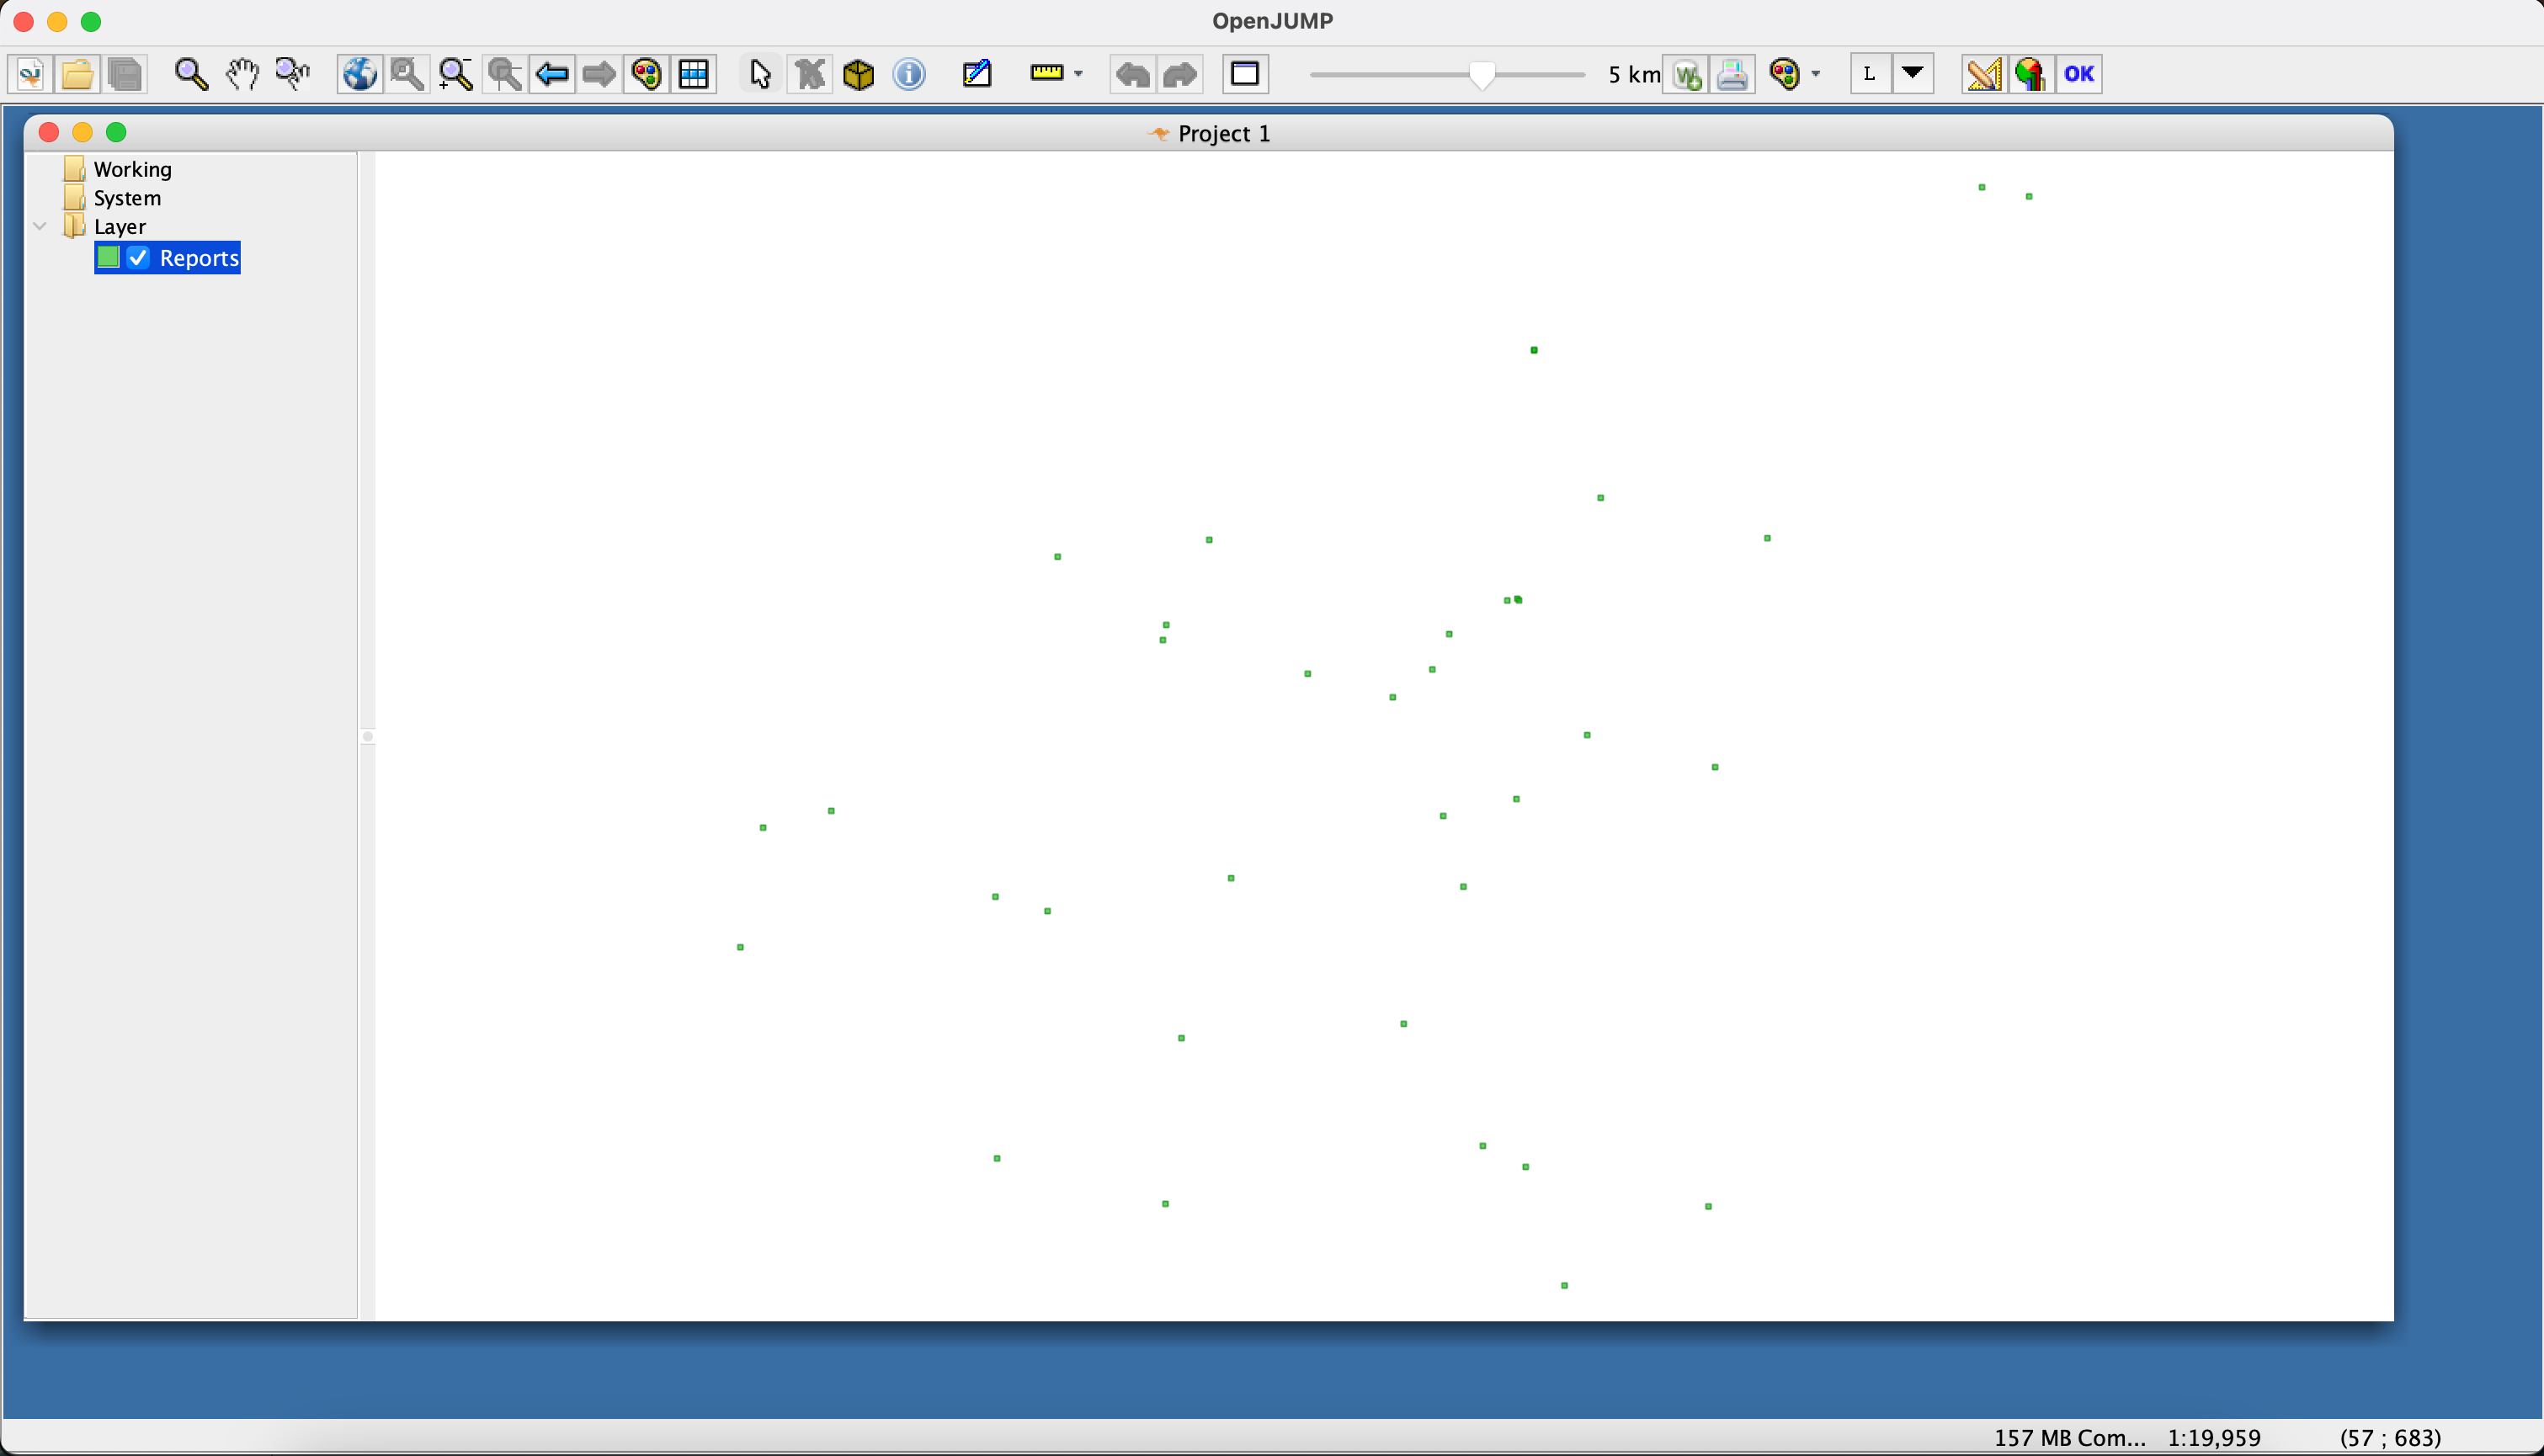
\includegraphics[width=0.8\textwidth]{images/oj_layer.png}
        \caption{Show report}
        \label{ER}
 \end{figure}

    \item\textbf{Route.java}
    It computes the road route and displays it as a LineString. 
    \begin{figure}[h]
        \centering
        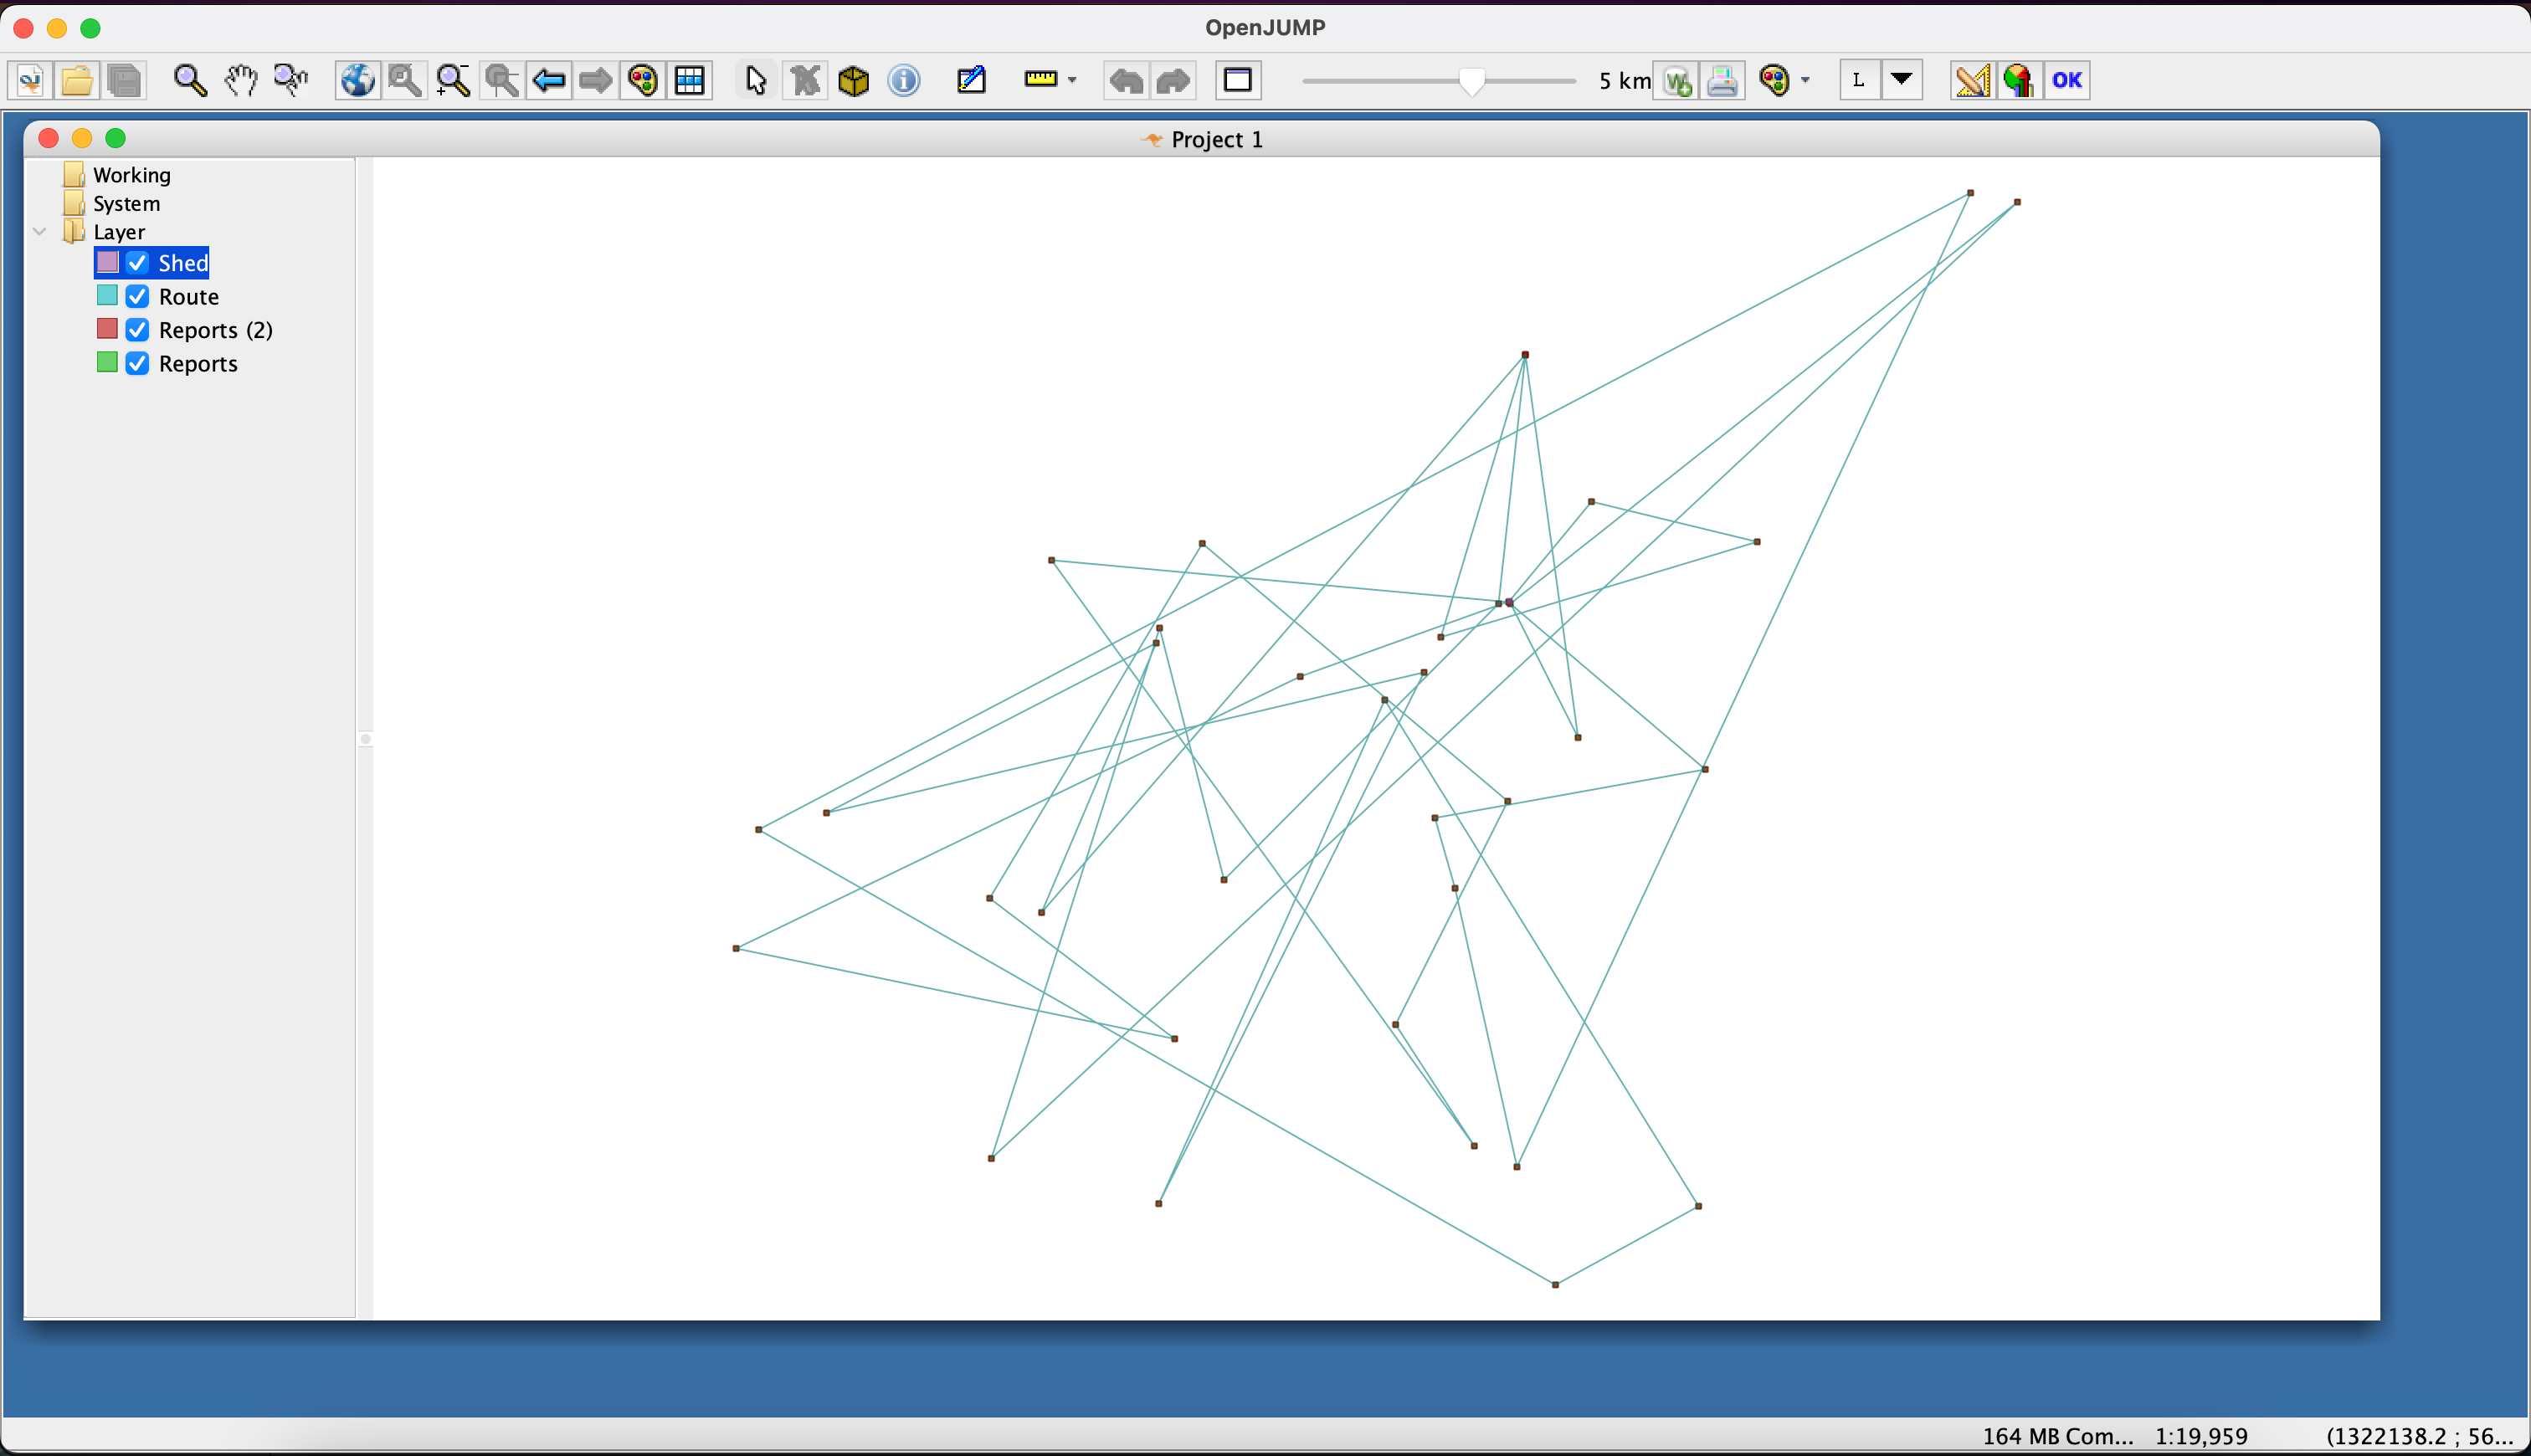
\includegraphics[width=0.8\textwidth]{images/oj_route.png}
        \caption{Route computed}
        \label{ER}
 \end{figure}
    

    \item \textbf{Export.java}
    This class is used to export the road route computed into a kml file to show it on google earth.
\end{itemize}
We will use OpenJUMP as GIS desktop software: the open source nature of OpenJUMP grants us the full accessibility of its interfaces for 2D geometry manipulation. The Output layers will be located in the ”Result” folder. The plugin will work as follows:
\begin{enumerate}
    \item The technician will launch the plugin.
    \item The technician chooses if he/she wants to load all reports or compute the road route and then the plugin will ask him to login to the system.
    \item If the technician chooses to show the reports, then the plugin will load the layer of all reports received.
    \item Otherwise, the plugin will compute the road route showing it as a LineString.
\end{enumerate}

\newpage
 \subsection{Database}
 
 \subsubsection{ER diagram}

 \begin{figure}[h]
        \centering
        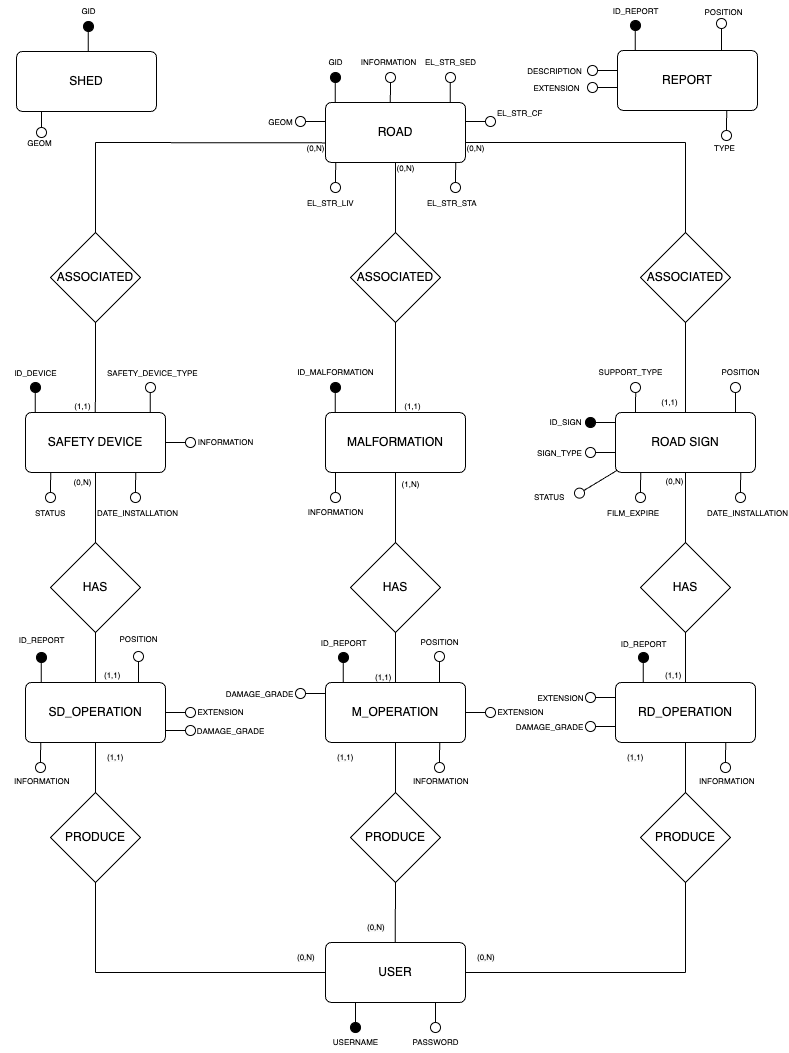
\includegraphics[width=0.8\textwidth]{images/ER.png}
        \caption{ER diagram}
        \label{ER}
 \end{figure}

 \newpage
 \subsubsection{Description of the Entities and the Relationship}
 In the Figure \ref{ER} are listed all the entities and relationship useful for the development of the system project.

 From the given shape files we have:
 \begin{itemize}
     \item \textbf{SHED}: this entity is associated with the position of the shed where the truck that carries out the road maintenance starts. This entity stores the given shed information provided by the customer document. 
     \item \textbf{ROAD}: this entity is referred to the geometries and informations of the Provincial road network. It stores the id of the road along with.
     Also this entity stores the given shed information provided by the customer document.
     
 \end{itemize} 
 The remaining entities are necessary to comply with the system specification: \textbf{USER} used to login the specialized team, enabling them to manage the road network informations. This entity is also used to store the authorized police officers that can query the state of the road infrastructure.
 \\
 The specialized team member can create three different types of report:
 \begin{itemize}
     \item \textbf{SD\_OPERATION}: report regarding the status of a specific safety device in a specific road. If a safety device needs to be replaced, the specialized team will insert the new date of installation of the new safety device and it has to be moved, the new position of the safety device. 
     Position is stored as geometry attribute of the \textbf{SAFETY DEVICE} entity. The date is automatically extracted from the device on which the report filling is taking place.
     The road sign is specified by the \textbf{SAFETY DEVICE} entity connected by the \textbf{HAS} relationship. 
     \item \textbf{M\_OPERATION}: report regarding information of a specific malformation present in a specific road. The malformation informations are associated to only \textbf{one} entry of the \textbf{MALFORMATION} entity. When the team goes there to inspect the road, it inserts the coordinates of where the damage is present in that specific road. Here it is also stored the position of a malformation since a malformation could be associated to more than one intervention: same damage to the road surface in different times.
     \item \textbf{RD\_OPERATION}: this report is used to signal the presence of alteration to a specific road sign of a road. The road sign report is referred to only \textbf{one} road sign defined by the \textbf{ROAD SIGN}. The road sign is associated with support type, the type of the signal that it is referring to, when its film will expire and when it was installed. Each road sign is associated to a position stored in geometry column, inserted by the specialized team when it installed the signal.
     If a road signal needs to be replaced, its corresponding entry is the \textbf{ROAD SIGN} table is updated with the new date of installation. 
 \end{itemize}
    The Date attribute of the three above entities, stores the date on which the report filling made by the specialized team has been made.
 
 Each one of these entities stores the information regarding a specific \textit{road sign}, \textit{safety device} and \textit{malformation} through out the time.\\
 Each user can create more reports, but each report is associated only to a specific user.  

 The citizens creates a new \textbf{REPORT} specifying: the \textit{position}, \textit{extension} of the damage, a brief \textit{description} and the \textit{type} of road object that he/she wants to make a report for. The types are associated to: \textit{road sign}, \textit{safety device} and \textit{malformation}.
 

 \subsubsection{Data Volumes and Redundancy}
 To ensure better redundancy of the data that will be inserted into the database, the following design choice has been applied:
 separate the general operation carried out by the specialized team when it will expect the road network, into three ad-hoc operation associated to each one of the above described road entity ( ROAD SIGN, SAFETY DEVICE, MALFORMATION). 
 This techniques has the following advantages:
 \begin{itemize}
     \item it implies replicating of data of the same type to ensure fault-tolerance
      \item the query time is lower with the respect to a single table because the number of entries to scan are only associated to the specific road object that it wants to know information about. When the member of the team would like to query a specific road object, it will query the \textit{report} table to know the type and its position, in order to organize its maintenance.
      \item it also helpful to understand which tables is larger and to increase only its STORAGE MEMORY accordingly.
 \end{itemize}
Regarding the amount of database access, it is necessary the creates indexes for the following tables to speed up the response time:
\begin{itemize}
    \item \textbf{REPORT}: since the Padova province has a not indifferent number of citizens, index here is crucial to not make the people wait when they submit the reports, to not ruin the user experience.
    \item \textbf{ROADS}: each road is associated to at least a malformation, road sign or safety device entry: to not slow down the operation required and possibly overload of the database server, the index would be important for the overall system health.
\end{itemize}
 \subsubsection{Security}
 In the Database, data before that is going to be insert into the database is properly sanitized and check validated, to ensure no potential threats can cause problems to the Database server, i.e. SQL Injection. 